
% \subsection{Applications}

% The fitting procedure has been employed to reproduce thermo-desorption experiments performed on Tungsten, EUROFER, Aluminium and Beryllium.


\subsubsection{Validation on tungsten}

The TDS spectrum measured by Ogorodnikova \textit{et al} \sidecite{ogorodnikova_deuterium_2003} has been reproduced by setting all traps parameters as free parameters.
The fitting procedure has been run for several numbers of traps as shown on Figure \ref{fig:number of traps comparison}.
It is clear that setting only one trap is not sufficient to reproduce the experimental data.
The two traps case shows better results but also has a discrepancy near \SI{600}{K}.
This discrepancy is removed when setting a third extrinsic trap to the simulation.

For this last case, the five free parameters are the detrapping energies $E_{p, 1}$, $E_{p, 2}$, $E_{p, 3}$ and densities $n_1$, $n_2$ (the third trapping site being created during the implantation, for which the creation parameters are not part of the free parameters and taken from \cite{ogorodnikova_deuterium_2003} or \sidecite{hodille_macroscopic_2015}).
This optimisation case is therefore a 5D optimisation problem.
Every other parameter is taken from \cite{hodille_macroscopic_2015}.
The resulting fit is shown on Figure \ref{fig:5D TDS} alongside with the contribution of each trap to the total spectrum.
An interesting feature of this spectrum is the negative area of the contribution of the second trap around \SI{400}{K}.
Because not all of these traps are saturated, when trap 1 is empyting, some of the hydrogen particles are nearly instantly trapped in the second trap which has a higher detrapping energy.

% (1 trap [ 0.88368005  1.44347635] 2 traps [ 0.83582125  1.23768655  0.98708714  6.85457283])
\begin{figure*} [h!]
    \centering
        \begin{subfigure}[t]{0.5\linewidth}
            \centering
            \captionsetup{width=.9\linewidth}
            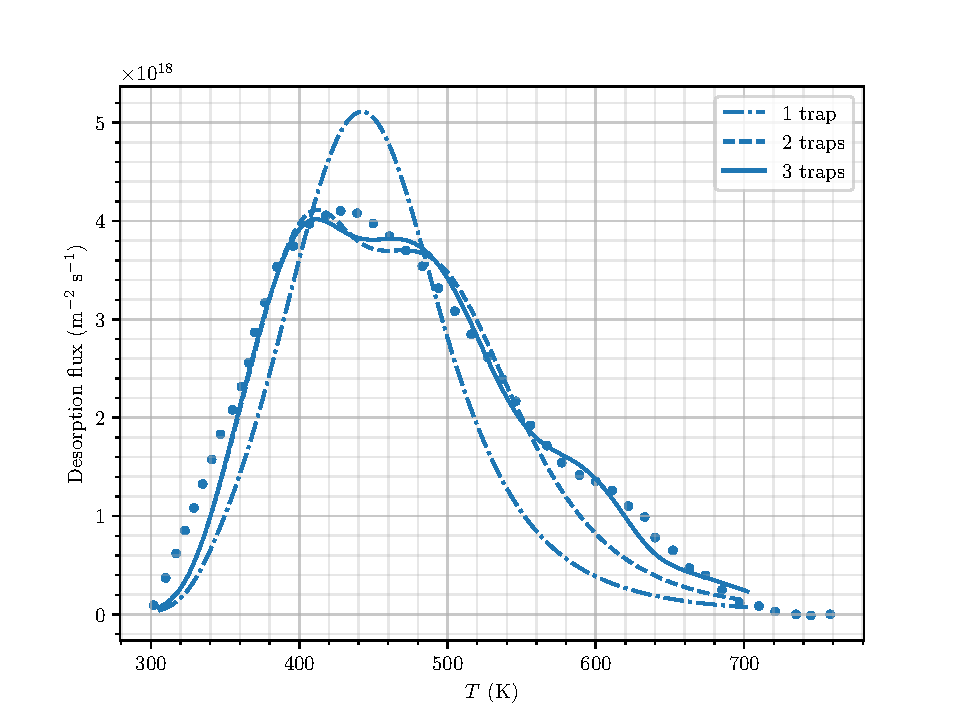
\includegraphics[width=\linewidth]{Figures/Chapter3/Parametric_optimisation/number_of_traps.pdf}
            \caption{Comparison of the resulting fit with several numbers of traps in the simulation.}
            \label{fig:number of traps comparison}
        \end{subfigure}%
        \begin{subfigure}[t]{0.5\linewidth}
            \centering
            \captionsetup{width=.9\linewidth}
            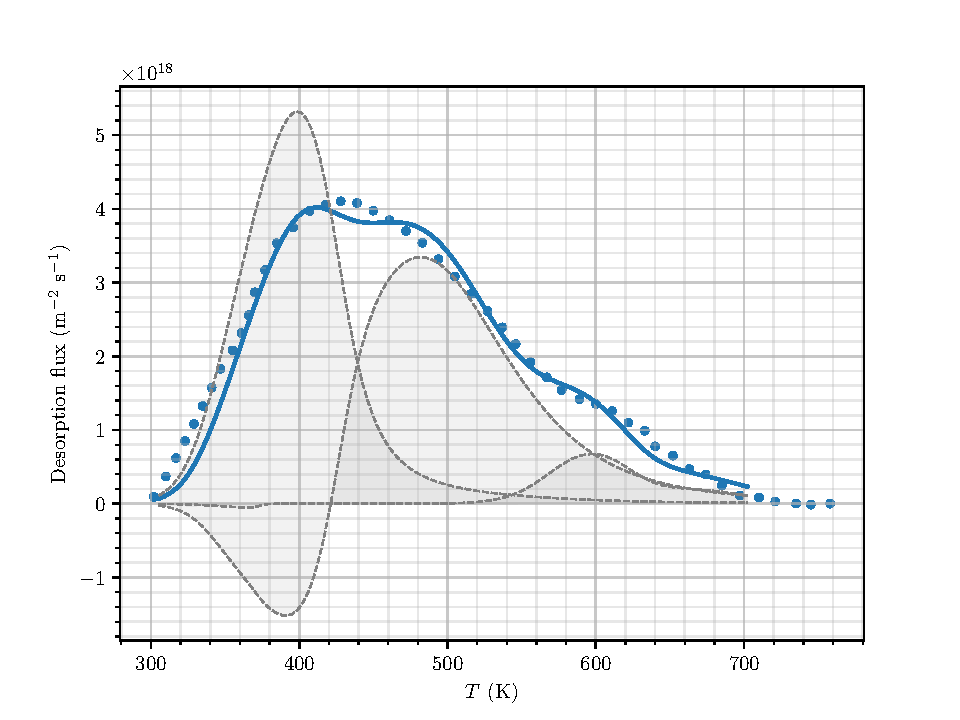
\includegraphics[width=\linewidth]{Figures/Chapter3/Parametric_optimisation/Ogorodnikova_5D.pdf}
            \caption{Identified by the fitting procedure with $E_1 = \SI{0.83}{eV}$, $E_2 = \SI{0.97}{eV}$, $E_3 = \SI{1.51}{eV}$, $n_1 = \SI{1.18e-3}{at.fr.}$ and \newline $n_2 = \SI{7.22e-4}{at.fr.}$.  Dashed lines correspond to the temporal evolution of each trapping population's inventory.}
            \label{fig:5D TDS}
        \end{subfigure}%
    \caption{Fitting TDS spectrum performed on Tungsten by Ogorodnikova \textit{et  al} \cite{ogorodnikova_deuterium_2003}. Dots correspond to experimental data.}
    \label{fig:TDS ogorodnikova}
\end{figure*}
The identified parameters are similar to the ones found by Hodille \textit{et al.} in \cite{hodille_macroscopic_2015}.
The total fitting procedure took a few hundred of cost function evaluations.
One single cost function evaluation "costing" less than \SI{20}{s} to compute (for that specific case), the total procedure lasted less than \SI{3}{h}.

% \subsubsection{EUROFER}

% Hollingsworth \textit{et al} performed thermo-desorption on pre-damaged EUROFER at several damage levels \sidecite{hollingsworth_comparative_2019}.
% Three spectra with similar exposure conditions have been fitted with one trapping site (since only one peak appears on the spectra) as shown on Figure \ref{fig:TDS EUROFER}.

% \begin{figure} [h!]
%     \centering
%     \includegraphics[width=0.9\linewidth]{Figures/Chapter3/Parametric_optimisation/EUROFER_hollingsworth.pdf}
%     \caption{TDS spectra of damaged EUROFER \cite{hollingsworth_comparative_2019}. Fitted with one trapping site (solid line) $E=\SI{1.06}{eV}$ and densities of \SI{8.9e-3}{at.fr}, \SI{2.8e-2}{at.fr} and \SI{5.0e-2}{at.fr} for \SI{0}{dpa}, \SI{0.01}{dpa} and \SI{0.1}{dpa}, respectively. Dashed lines correspond to optimisations with an unweighted cost function. Dots correspond to experimental data.}
%     \label{fig:TDS EUROFER}
% \end{figure}

% To put the emphasis on peaks, a weighting factor of 10 has been applied for $T \in [\SI{445}{K}, \SI{492}{K}]$.
% Not applying this factor near the peak region results in a closer fit in other regions but a higher peak value.
% The identified trap energy is $E_p$ \SI{1.06}{eV} for all spectra whereas the trap density $n$ is \SI{8.9e-3}{at.fr} for the undamaged sample, \SI{2.8e-2}{at.fr} for \SI{0.01}{dpa} and \newline \SI{5.0e-2}{at.fr} for \SI{0.1}{dpa}.
% For all simulations the attempt frequency $p_0$ is \SI{1e13}{s^{-1}} and the diffusion coefficient is taken from \sidecite{esteban_hydrogen_2007}.

% The total fitting procedure took less than two hours for fitting the three spectra.
% A more thorough study of these experiments could involve constraining the algorithm with profilometry data obtained by Hollingsworth \textit{et al} \cite{hollingsworth_comparative_2019}.
% Indeed, having a non-homogeneous trapping site distribution could help having a better fit of both the profilometry data and the TDS spectra. 

% \subsubsection{Aluminium}

% The experiment performed on Aluminium by Quiros \textit{et al} \sidecite{quiros_blistering_2019, quiros_blister_2017} has also been reproduced with FESTIM.

% Only one trap has been set in the simulation and its energy $E_p$ and density $n$ are set as free parameters.
% Every other parameters are fixed and taken from \cite{quiros_blister_2017, quiros_blistering_2019}.
% The resulting simulated TDS spectrum is shown on Figure \ref{fig:TDS alu}.
% \begin{figure} [h!]
%     \centering
%     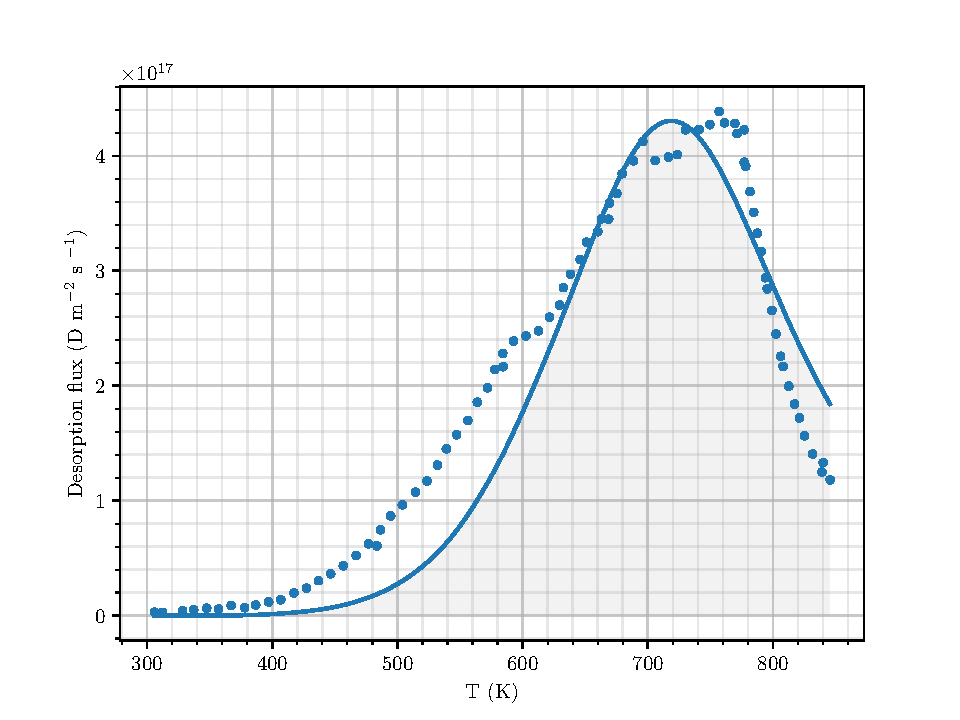
\includegraphics[width=0.9\linewidth]{Figures/Chapter3/Parametric_optimisation/alu_quiros.pdf}
%     \caption{TDS spectrum of aluminium exposed to \SI{3e23}{H.m^{-2}} at \SI{618}{K} \cite{quiros_blister_2017, quiros_blistering_2019}. Fitted with one trapping site $n = \SI{1.8e-2}{at.fr.}$ and $E =\SI{1.1}{eV}$. Dots correspond to experimental data. Dashed lines correspond to the temporal evolution of each trapping population's inventory.}
%     \label{fig:TDS alu}
% \end{figure}


% The identified parameters are $n = \SI{1.8e-2}{at.fr.}$ and $E =\SI{1.1}{eV}$.
% The trapping sites density is significantly higher than the one described in \cite{quiros_blister_2017}.
% However, the TDS spectrum obtained with this procedure better fits the experimental data since the one obtained by Quiros \textit{et al} requires a 10-fold increase.
% The fitting procedure took less than a hundred cost function evaluations, which corresponds in total to a few dozens of minutes.

% \subsubsection{Beryllium}
% Be co-deposition experiments performed by Baldwin \textit{et al} \sidecite{baldwin_experimental_2014} were reproduced.
% In this experiment, a \SI{1}{\micro m} thick Be-D layer is grown on Tungsten at \SI{330}{K}. 
% Following the strategy proposed by Baldwin \textit{et al}, only the thermo-desorption phase has been simulated with two trapping sites with homogeneously distributed densities and with initial occupancies $f_i$.
% There are therefore three free parameters per trap (energy, density and initial occupancy) which makes this optimisation problem 6D.
% It is assumed that the surface flux is the net balance between incoming flux from the chamber (very low since the pressure is $\SI{1}{\micro Pa}$) and the molecular recombination flux.
% All the other parameters are described in \cite{baldwin_experimental_2014}.

% The resulting optimised TDS spectrum is shown on Figure \ref{fig:TDS baldwin}.
% The optimised parameters are $E_{p, 1} = \SI{0.75}{eV}$, $n_1 = \SI{1.09e-1}{at.fr.}$, $f_1=0.73$, $E_{p, 2} = \SI{0.93}{eV}$, \newline ${n_2 = \SI{3.40e-2}{at.fr.}}$, $f_2=0.28$.
% These values are in agreement with the ones found by Baldwin \textit{et al} \cite{baldwin_experimental_2014} and took only a few of minutes to compute since the implantation phase was not simulated.

% \begin{figure} [h!]
%     \centering
%     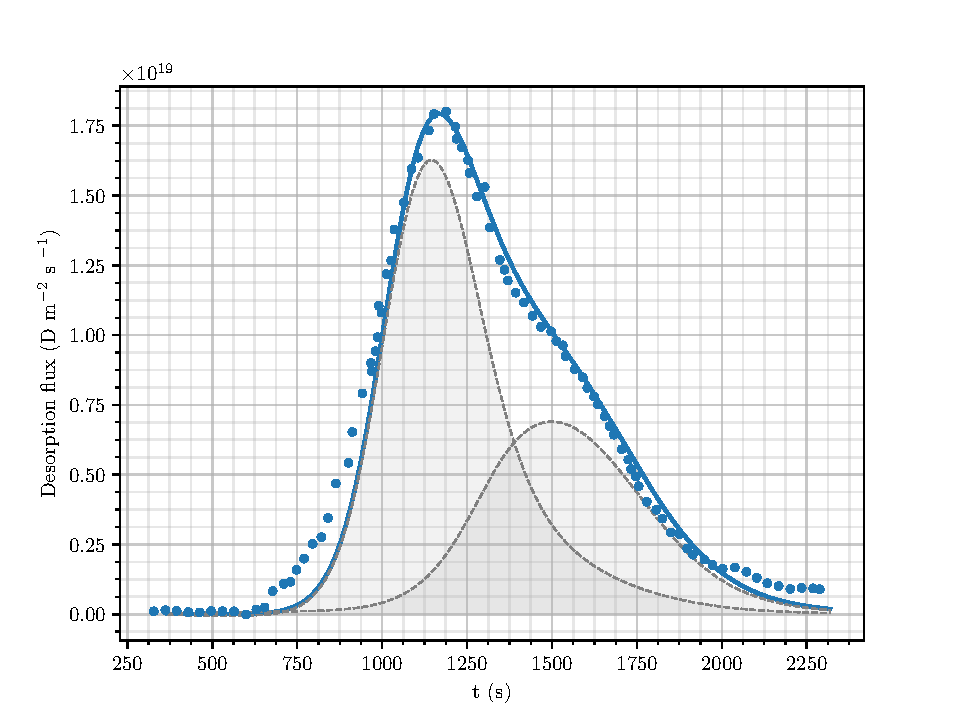
\includegraphics[width=0.9\linewidth]{Figures/Chapter3/Parametric_optimisation/baldwin_be.pdf}
%     \caption{TDS spectrum of co-deposited Be-D \cite{baldwin_experimental_2014} simulated with two trapping sites. Dots correspond to experimental data.}
%     \label{fig:TDS baldwin}
% \end{figure}

\subsubsection{Limitations}

Even though an automated technique is proposed, the user still has some choices to make in order to ensure the credibility of the fitted spectrum.
As shown on Figure \ref{fig:TDS EUROFER}, weighting the cost function near regions of interest will result in a better fit in these regions.
Users should also be aware of the number of traps the data is being fitted with.
As shown on Figure \ref{fig:number of traps comparison} too few traps in the simulation will not result in a satisfactory fit (even though the optimisation routine will converge to an optimised solution).
Moreover, as shown on Figure \ref{fig:hurley_comparison}, one single TDS spectrum can be reproduced with several traps of different energies and densities.
This means that the cost function with several traps as free parameters can have several local minima of very similar values.
Adding traps to an optimisation problem can also help having a better fit of the experimental data in some cases.
But artificially adding more and more traps is not necessarily realistic and could lead to misinterpretation of the results.

\begin{figure}[h!]
    \centering
    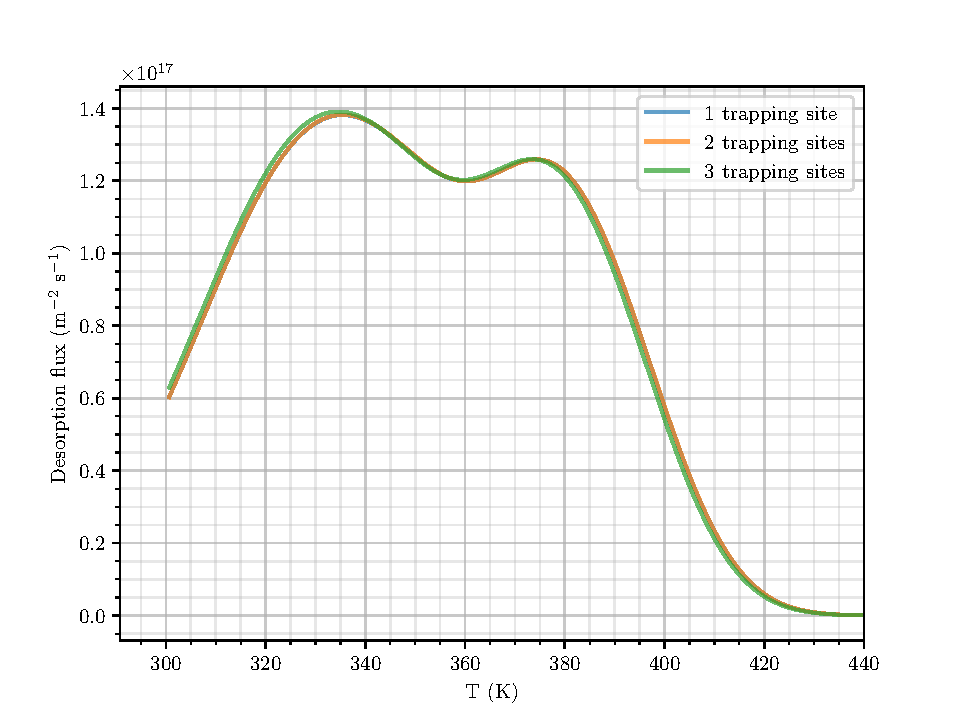
\includegraphics[width=0.9\linewidth]{Figures/Chapter3/Parametric_optimisation/hurley_comparison.pdf}
    \caption{TDS spectrum reproduced with several sets of parameters showing the existence of several solutions to a single optimisation problem.}
    \label{fig:hurley_comparison}
\end{figure}

In the first case with only one trapping site, as described by Hurley \textit{et al} in \sidecite{hurley_numerical_2015}, the binding energy is \SI{0.55}{eV} and the trap density is \SI{2.08e24}{m^{-3}}.
The appearance of two peaks is due to the desorption on different sides of the sample as explained in \cite{hurley_numerical_2015}.
In the second case, the curve as been reproduced with two trapping sites which energies and densities are respectively \SI{0.51}{eV} and \SI{0.57}{eV} and \SI{2.02e24}{m^{-3}} and \SI{2.12e24}{m^{-3}}.
In the third case, it has been reproduced with three trapping sites which energies and densities are respectively \SI{0.55}{eV}, \SI{0.38}{eV} and \SI{0.51}{eV} and \SI{2.12e24}{m^{-3}}, \SI{2.26e24}{m^{-3}} and \newline \SI{2.13e24}{m^{-3}}.

This example illustrates how a single spectrum can be simulated with several sets of parameters by varying the number of traps in the simulation.
One way to avoid this from happening is to have a set of experiments with varying parameters such as the implantation temperature, the heating ramp, the fluence, dwelling time before TDS, etc.
